%%----------------cost vs. threshold--------------------
%\begin{figure*}
%  \centering
%  \subfloat[\covtype]{
%  \centering 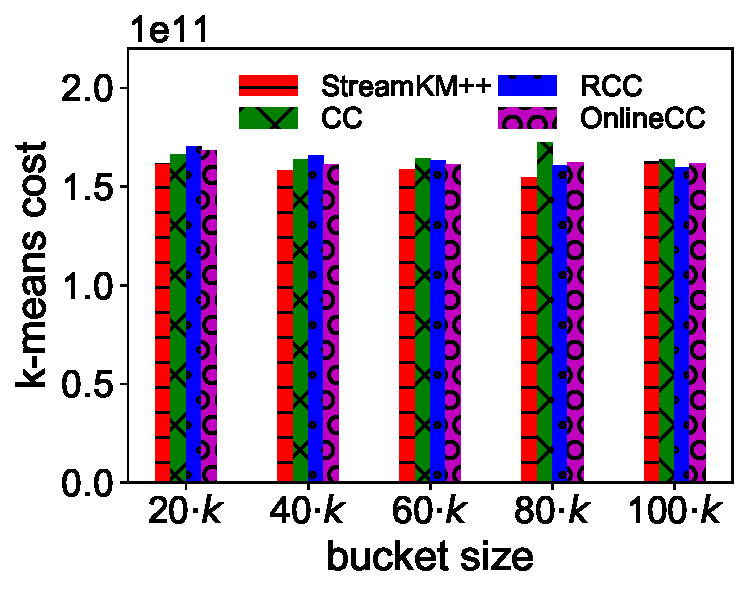
\includegraphics[width=0.23\textwidth]{expfigs/accuracy_bucketsize/covtype_cost_vs_m.pdf}
%  }
%  \subfloat[\power]{
%  \centering 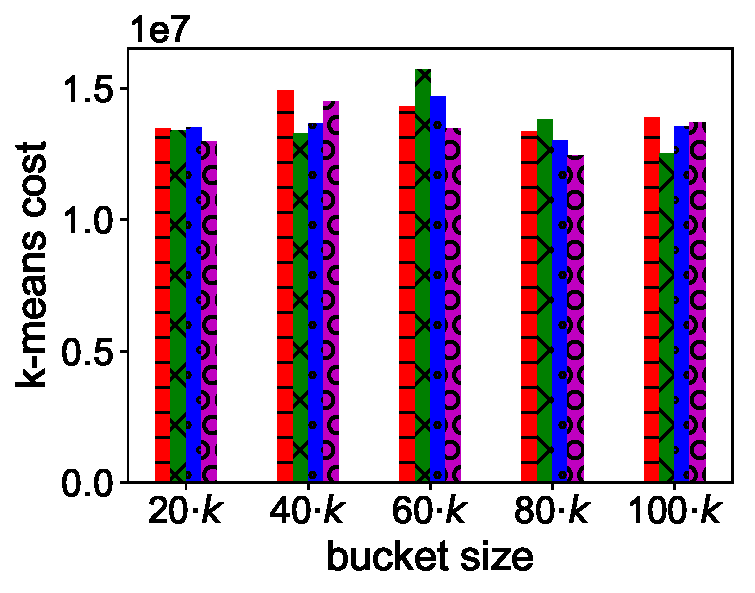
\includegraphics[width=0.23\textwidth]{expfigs/accuracy_bucketsize/power_cost_vs_m.pdf}
%  }
%  \subfloat[\intrusion]{
%  \centering 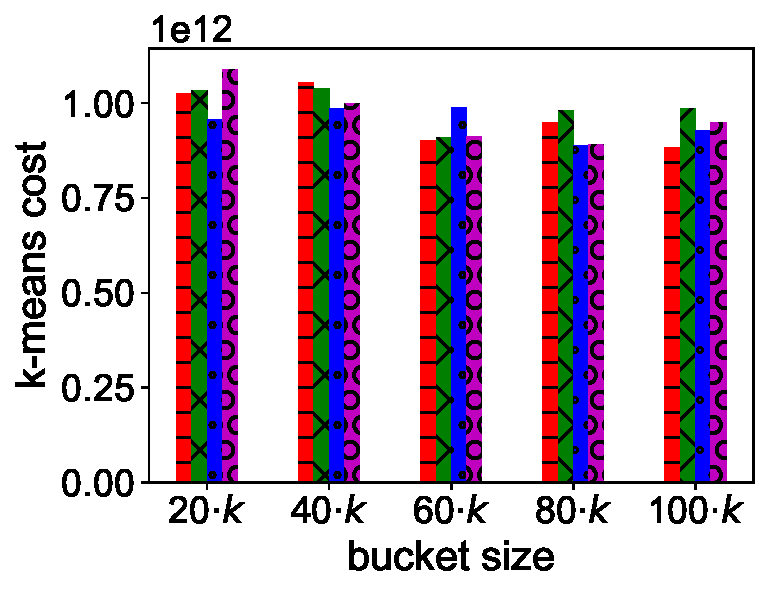
\includegraphics[width=0.23\textwidth]{expfigs/accuracy_bucketsize/intrusion_cost_vs_m.pdf}
%  }
%  \subfloat[\drift]{
%  \centering 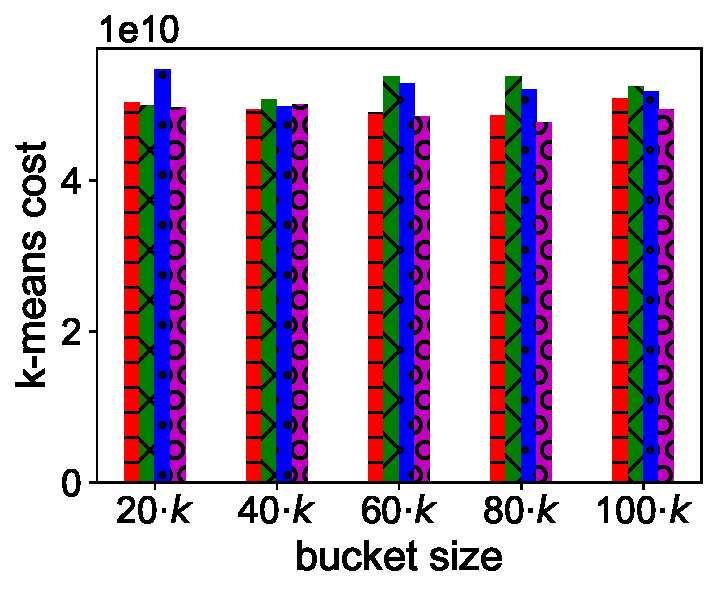
\includegraphics[width=0.23\textwidth]{expfigs/accuracy_bucketsize/synthetic_cost_vs_m.pdf}
%  }
%  \caption{\km cost vs. bucket size $m$. The cost is computed at the end of observing all the points. The number of clusters $k=30$, query interval $q=100$.  }
% \label{fig:cost-versus-m}
%\end{figure*}
%%----------------

%----------------time vs. threshold--------------------
\begin{figure*}
  \centering
  \subfloat[\covtype]{
  \centering 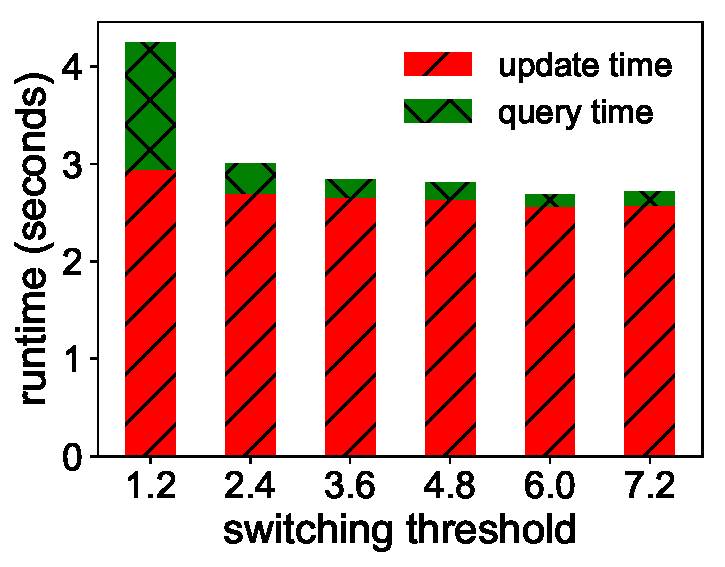
\includegraphics[width=0.23\textwidth]{expfigs/onlinecc_time/covtype_time.pdf}
  }
  \subfloat[\power]{
  \centering 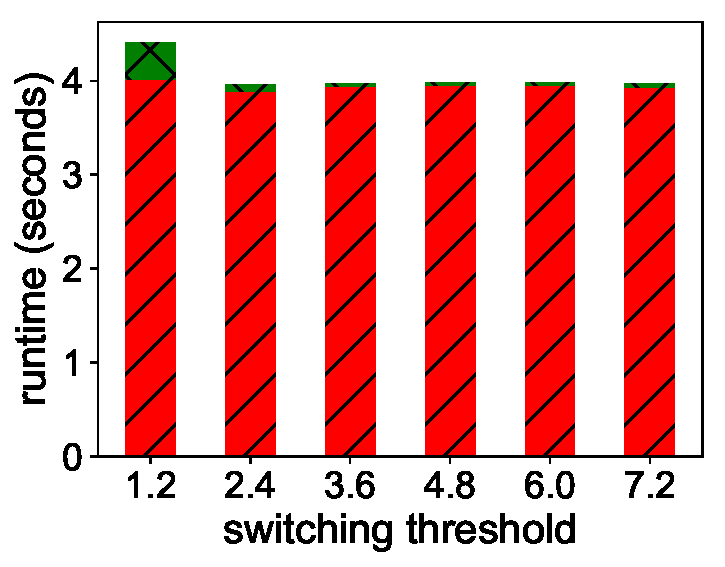
\includegraphics[width=0.23\textwidth]{expfigs/onlinecc_time/power_time.pdf}
  }
  \subfloat[\intrusion]{
  \centering 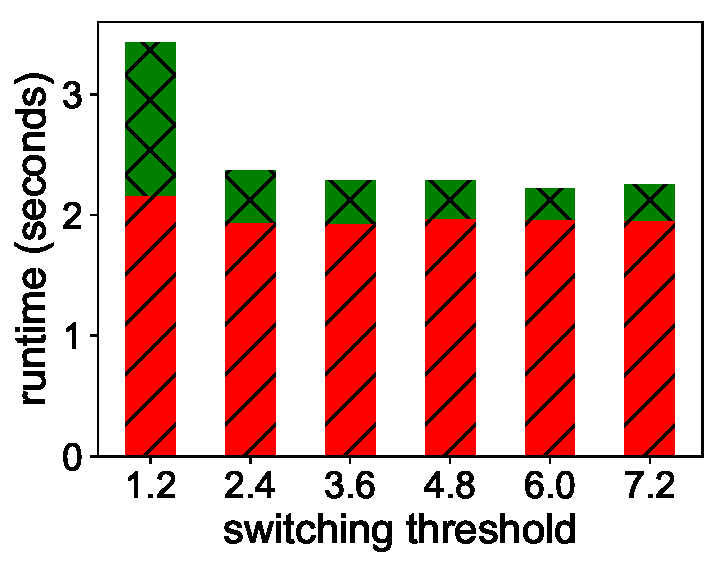
\includegraphics[width=0.23\textwidth]{expfigs/onlinecc_time/intrusion_time.pdf}
  }
  \subfloat[\drift]{
  \centering 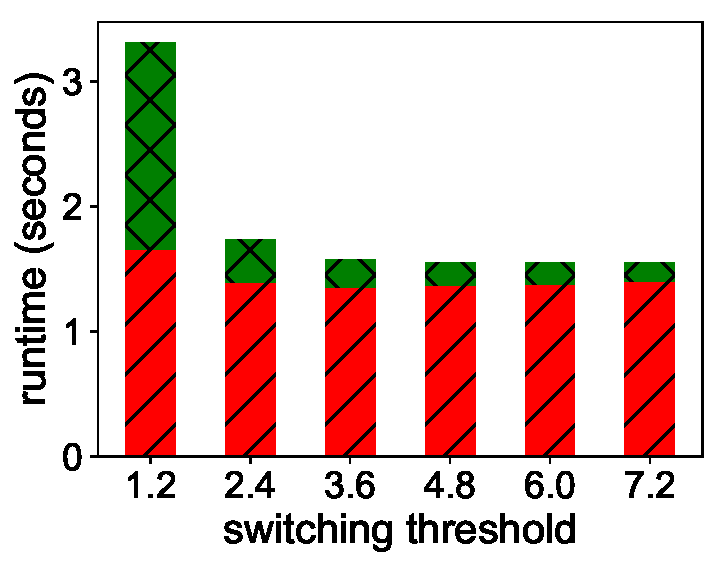
\includegraphics[width=0.23\textwidth]{expfigs/onlinecc_time/synthetic_time.pdf}
  }
  \caption{Total runtime (seconds)  vs. switch threshold $\alpha$ in \hybrid algorithm. 
  The number of clusters $k=30$, query interval $q=100$.  
  The update and query time are both counted for the whole stream instead of per point.}
 \label{fig:time-versus-threshold}
\end{figure*}
%----------------